%!TEX root = ../../proposal.tex

% Write a brief summary of the proposal. The summary should not exceed 120 words and best be a paragraph long. The summary should include a few lines about the background information, the main research question or problem that you want to write about, and your research methods. The proposal summary should not contain any references or citations. Remember that your entire proposal cannot exceed 1500 words, so choose the words in this section carefully. The 1500 words you will write in the proposal document will exclude any words contained in the tables, figures, and references. You can use this template for writing your proposal.


%10-20 pages maximum

%Abstract
%Table of contents
%Introduction
%Background
%Goal and Objectives
%Methodology
%Timeplan
%Discussion/Conclusion
%Acknowledgements
%References
%Appendix

\clearpage

\section{Introduction}
\begin{body}
Micro computed tomography ($\mu$CT) is a widely used modality in industry and research. For the latter it enables the study of small structures in animals, for example rodents such as mice.\cite{percianoInsight3DMicroCT2017}.
A common task while performing short term or long term studies with mice is the segmentation of the image data, as it is a important step for quantitative image analysis\cite{sheppardTechniquesHelicalScanning2014}. Segmentation can be defined as the process of separating various image components and extracting parts that are of interest for later analysis\cite{percianoInsight3DMicroCT2017}.
\newline
There exist a few free and open-source programs capable of segmenting $\mu$CT datasets.
The two actively maintained and well known\cite{mandoliniComparisonThree3D2022,virziComprehensiveReview3D2020} software packages are:
\begin{itemize}
	\item[\ding{108}] \textsc{ITK-SNAP}\cite{yushkevichUserguided3DActive2006}
	\item[\ding{108}] \textsc{3D Slicer}\cite{kikinis3DSlicerPlatform2014}
\end{itemize}
Both provide the user with a plethora of segmentation algorithms and tools and are capable of complex segmentation workflows.
\end{body}

\section{Problem Statement}
\begin{body}
\lipsum[2-3]

\end{body}

\clearpage
\section{Objectives and Aims}
\begin{body}
\lipsum[2-3]

\end{body}
\clearpage
\section{Literature to be reviewed}
\begin{body}
The source of literature used for this master thesis are PubMed, ScienceDirect IEEE Xplore and the meta search engine Google Scholar. The main workflow of searching for appropriate literature was to search for publications covering the defined keywords\ref{s:Keywords} in the abstract, reading as many of the papers as possible and filtering out the most relevant.
The following papers are the result of this workflow at the current time:
\begin{itemize}
  \item[\ding{108}] Comparison of segmentation tools for structural analysis of bone tissues by finite elements (Argüello et al. \textsf{\textbf{Journal of Physics}})
  \item[\ding{108}] Comprehensive Review of 3D Segmentation Software Tools for MRI Usable for Pelvic Surgery Planning (Virzì et al. \textsf{\textbf{Journal of Digital Imaging}})
  \item[\ding{108}] Comparison of Three 3D Segmentation Software Tools for Hip Surgical Planning (Mandolini et al. \textsf{\bfseries{MDPI}})
  \item[\ding{108}] Morphological mouse phenotyping: anatomy, histology and imaging (Ruberte et al. \textsf{\bfseries{Academic Press}})
  \item[\ding{108}] User-guided 3D active contour segmentation of anatomical structures: Significantly improved efficiency and reliability (Yushkevich et al. \textsf{\bfseries{NeuroImage}})
  \item[\ding{108}] Medical image segmentation on GPUs – A comprehensive review (Smistad et al. \textsf{\bfseries{Medical Image Analysis}})
  \item[\ding{108}] Segmentation and Visual Analysis of Whole-Body Mouse Skeleton microSPECT (Khmelinskii et al. \textsf{\bfseries{PLoS ONE}})
  \item[\ding{108}] SlicerRT: Radiation therapy research toolkit for 3D Slicer (Pinter et al. \textsf{\bfseries{Medical Physics}})
  \item[\ding{108}] Insight into 3D micro-CT data: exploring segmentation algorithms through performance metrics (Perciano et al. \textsf{\bfseries{Journal of Synchrotron Radiation}})
  \item[\ding{108}] SAMM (Segment Any Medical Model): A 3D Slicer Integration to SAM (Liu et al. \textsf{\bfseries{Johns Hopkins University}})

\end{itemize}
\end{body}

\clearpage
\section{Research design and Methods}
\begin{body}
\lipsum[2-3]

\end{body}

\section{Outcome}
\begin{body}
  \lipsum[2-3]

\end{body}

\clearpage
\section{Study Period}
\subsection{Milestones}
\begin{body}
\begin{itemize}
	\item[\ding{110}] Find supervisor and topic in September 2023
	\item[\ding{110}] Submission of the abstract in November 2023
	\item[\ding{110}] Submission of the research proposal in February 2024
	\item[\ding{110}] Finishing Segmentation work in April 2024
	\item[\ding{110}] Finishing Guide evaluation at the end of May 2024
	\item[\ding{110}] Finish the first version of the thesis in June 2024
	\item[\ding{110}] Submission of the final thesis in July 2024
\end{itemize}
\end{body}

\subsection{Chart}
\begin{body}
The segmentation work and literature search is planned to be finished by the end of April 2024.
After the segmentation work is done the guide will be tested and evaluated from April 2024 until June 2024.
Writing of the thesis starts with February 2024 and should be finished by June or July 2024.
The final examination should at the latest take place in October 2024.
\newline
\newline
\noindent
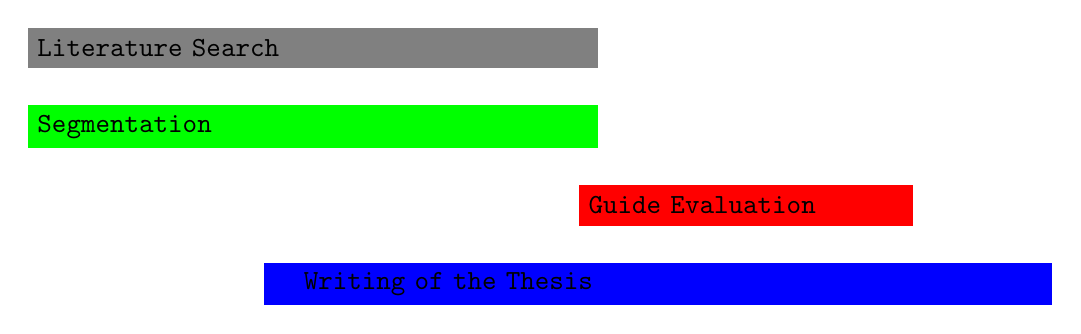
\begin{tikzpicture}
	\node at (0,0) [right=3cm,rectangle,draw=blue,fill=blue,minimum width=10cm,minimum height=0.5cm,text width=9cm] {\texttt{Writing of the Thesis}};
	\node at (0,3) [right=0cm,rectangle,draw=gray,fill=gray,minimum width=7cm,minimum height=0.5cm,text width=7cm] {\texttt{Literature Search}};
	\node at (0,2) [right=0cm,rectangle,draw=green,fill=green,minimum width=7cm,minimum height=0.5cm,text width=7cm] {\texttt{Segmentation}};
	\node at (0,1) [right=7cm,rectangle,draw=red,fill=red,minimum width=4cm,minimum height=0.5cm,text width=4cm] {\texttt{Guide Evaluation}};
\end{tikzpicture}
\newline
\noindent
\begin{tikzpicture}
	\draw [line width=0.5mm] (0,0) -- (15,0);
	  \foreach \x in {1,3,5,7,9,11,13}
	    \draw [line width=0.5mm](\x cm,5pt) -- (\x cm,-5pt);
	\draw (1,0) node[below=3pt] {$\begin{turn}{45}January 2024\end{turn}$};
	\draw (3,0) node[below=3pt] {$\begin{turn}{45}February 2024\end{turn}$};
	\draw (5,0) node[below=3pt] {$\begin{turn}{45}March 2024\end{turn}$};
	\draw (7,0) node[below=3pt] {$\begin{turn}{45}April 2024\end{turn}$};
	\draw (9,0) node[below=3pt] {$\begin{turn}{45}May 2024\end{turn}$};
	\draw (11,0) node[below=3pt] {$\begin{turn}{45}June 2024\end{turn}$};
	\draw (13,0) node[below=3pt] {$\begin{turn}{45}July 2024\end{turn}$};
\end{tikzpicture}
\end{body}
